\section{User documentation}

The following section contains user documentation for the \textit{Editor} application, following the scenarios from the \autoref{analysis} Analysis.
This section describes the basic features of the \textit{Editor} application and how to use it.

The documentation of the \textit{Runner} module is to be found in the \autoref{devDocs} Developer documentation, as there is no user interface for the \textit{Runner} module itself and the module is to be used only via its \ac{API} in code.

\subsection{Editor application}

The \textit{Editor} application is available as a web application.
To access the user interface, navigate to the URL of the running server instance using a modern web browser.
% If unsure, contact the administrator of your \textit{Editor} server instance. 
Instructions on how to setup the \textit{Editor} server instance are to be found in the \autoref{adminDocs} Administrator documentation.

\subsubsection{Getting started}

After accessing the \textit{Editor} application, the user is greeted by a welcome screen.
From here, they can choose whether to create new blank automation or to load existing automation from their device.
In case the uploaded file is not a valid workflow definition, the user is informed about the reason and asked to try again.

\begin{figure}[!h]
    \begin{center}
        \fbox{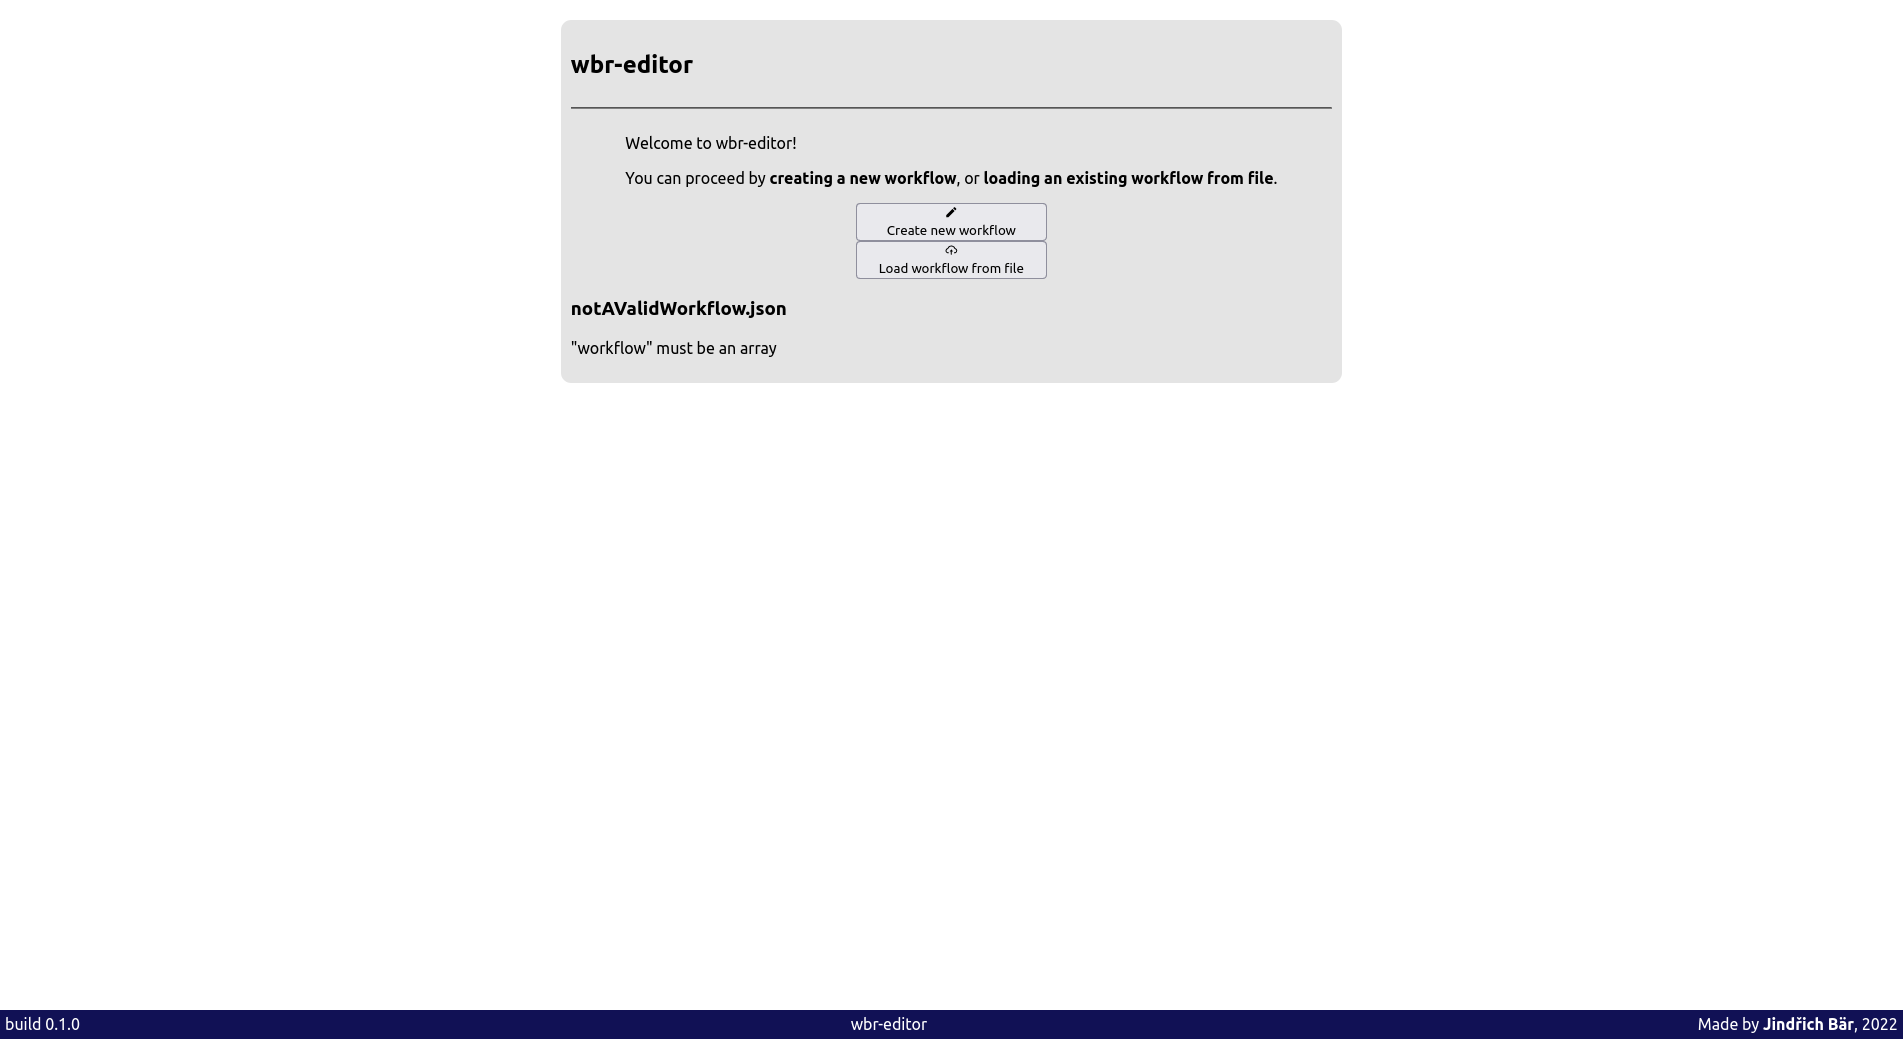
\includegraphics[width=0.75\textwidth]{./img/tutorial/initial.png}}
    \end{center}
    \caption{The initial screen}
\end{figure}
\clearpage

\subsubsection{Adding rules}
As described in the \autoref{formatDesign} Workflow definition format, the workflow definition file is a JSON file,
consisting of \textit{Rules} - \textit{Conditions} and their matching \textit{Actions}.

The user can add a new blank pair to the workflow definition file by clicking the blue square \texttt{`+'} (\textit{Plus}) button
in the bottom of the workflow editor.

\begin{figure}[!h]
    \begin{center}
        \fbox{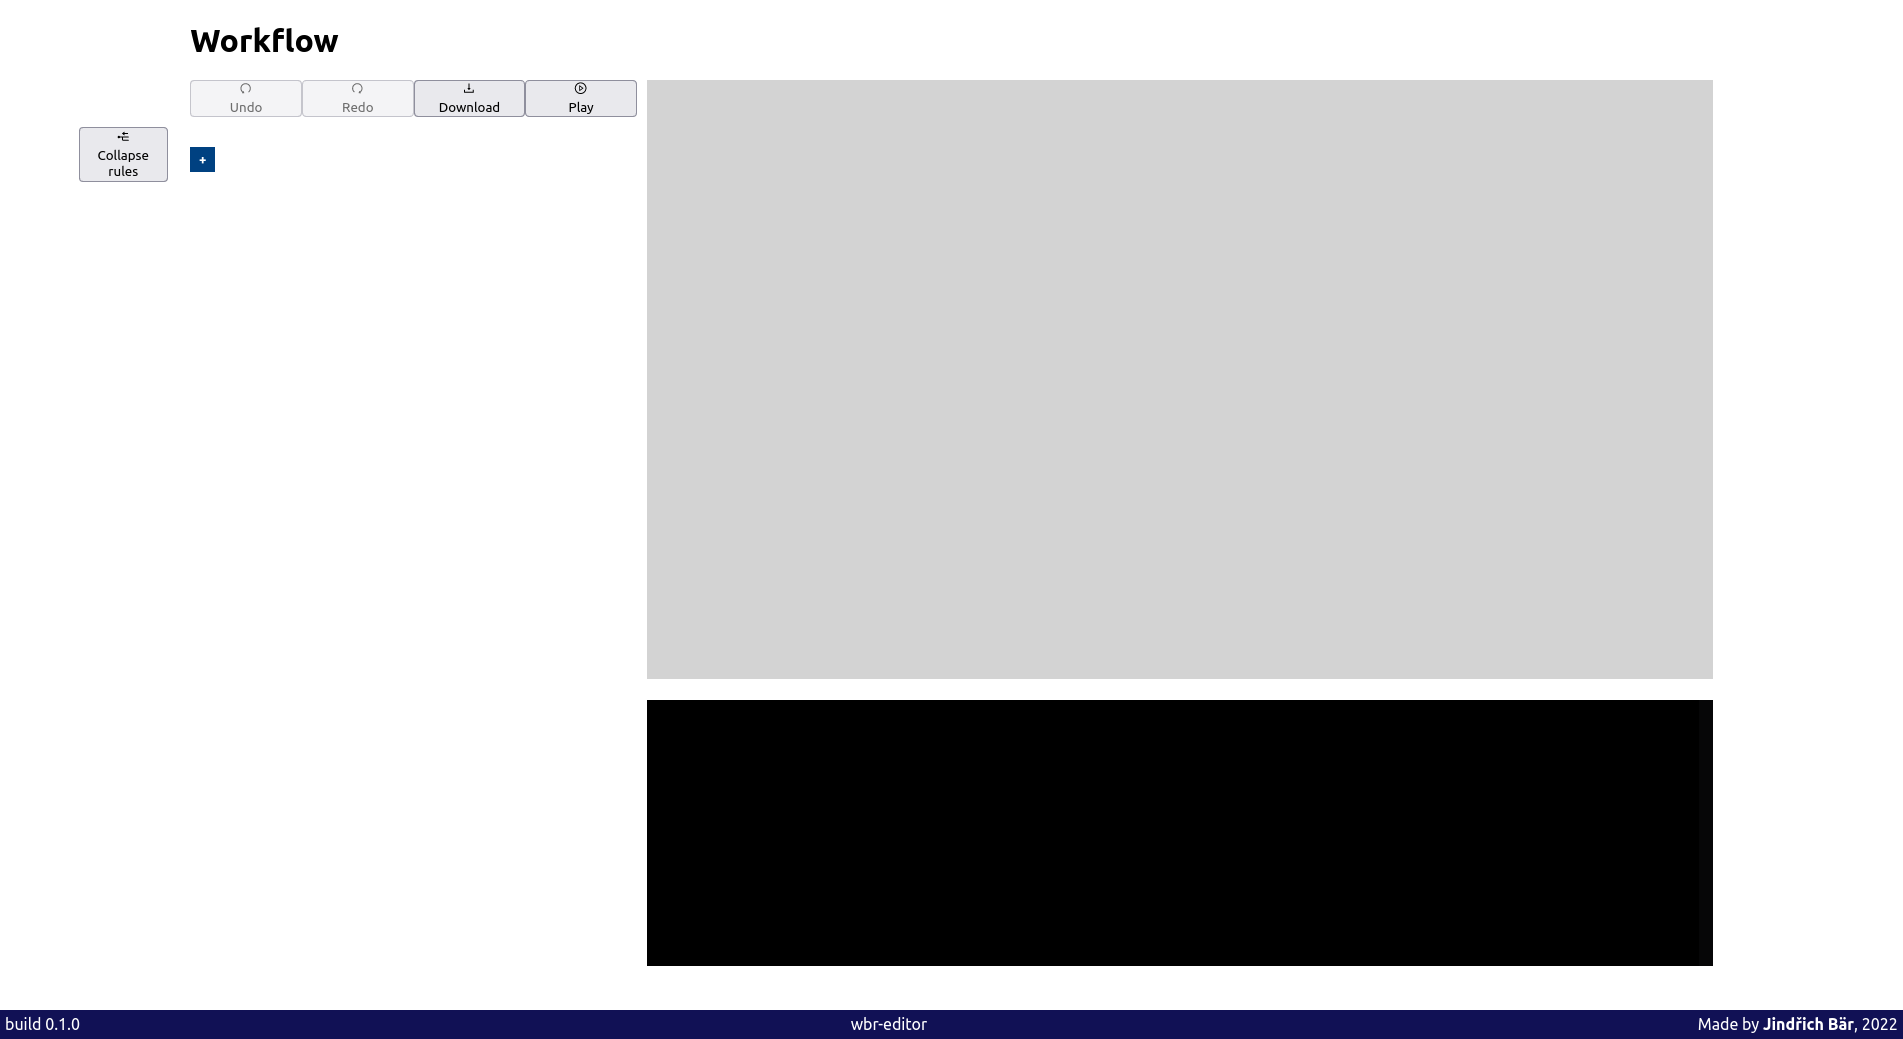
\includegraphics[width=0.75\textwidth]{./img/tutorial/blank.png}}
    \end{center}
    \caption{The workflow editor with a new blank workflow}
\end{figure}

After clicking the \texttt{`+'} button, the currently edited workflow is updated,
appending the new blank pair to the end of the workflow definition. 
Clicking the \texttt{`+'} button repeatedly adds new blank pairs to the end of the workflow definition.

\begin{figure}[!h]
    \begin{center}
        \fbox{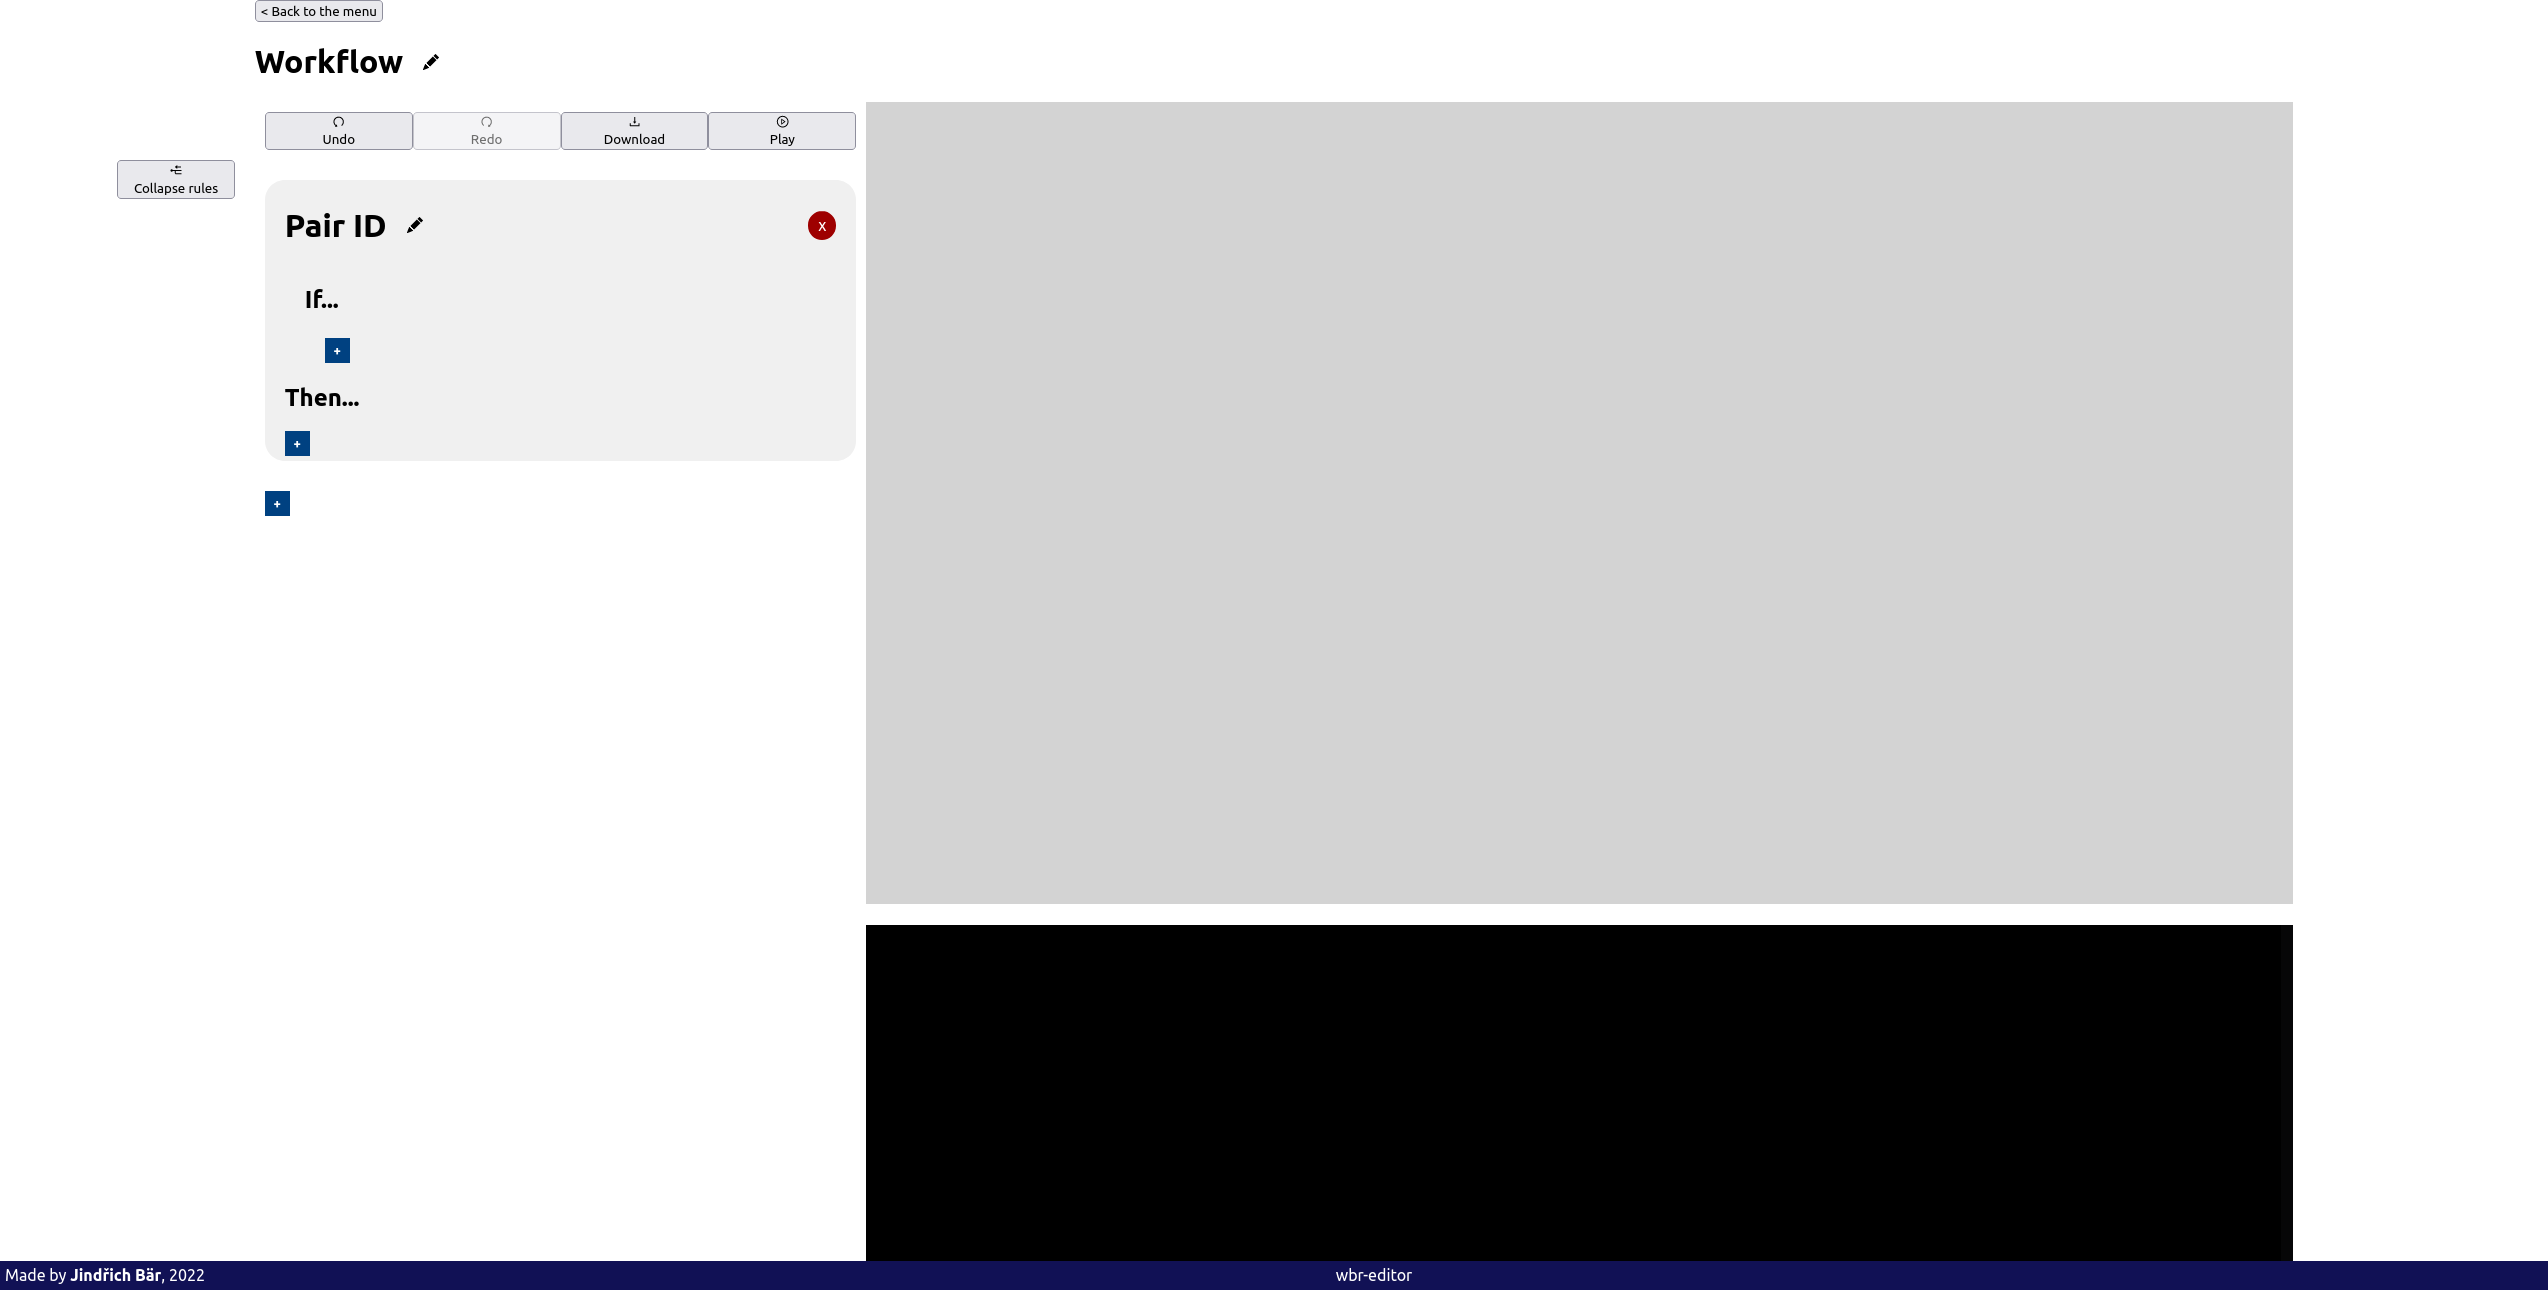
\includegraphics[width=0.75\textwidth]{./img/tutorial/newPair.png}}
    \end{center}
    \caption{A new blank pair is added to the workflow}
\end{figure}

Unwanted pairs can be removed by clicking the red round \texttt{`x'} button in the top right corner of the pair editor.
In such case, the workflow is updated and the pairs under the removed one are are shifted up.
\clearpage
\subsubsection{Editing the conditions}

As stated in the \autoref{formatDesign}, Workflow definition format, the pairs are defined as \textit{Conditions} and \textit{Actions}.
The automation interpreter is able to find the matching condition for the current state of the browser and execute the corresponding set of actions.

The pair's \textit{Condition} is displayed under the section ``If'' in the workflow editor.
The condition is defined as a possibly nested tree of simple condition expressions and logical operators.

By default, the condition consists of one empty \texttt{\$and} operator. 
This operator is used to combine the nested conditions - all of the nested conditions must be true for the pair to be true.
Removing this default operator will result in creating an empty clause - a condition that is always true.
This is useful e.g. for defining a default set of actions.

The conditions can be specified by clicking the blue square \texttt{`+'} button in the bottom of the operator section.

\begin{figure}[!h]
    \begin{center}
        \fbox{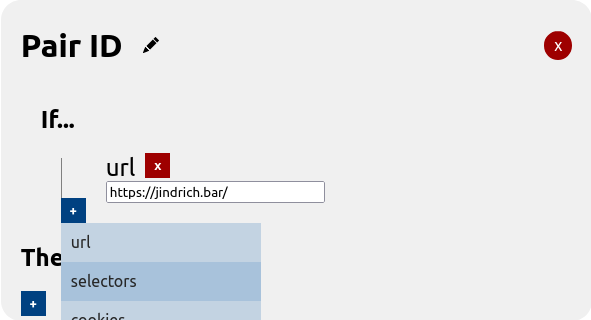
\includegraphics[width=0.60\textwidth]{./img/tutorial/and.png}}
    \end{center}
    \caption{Specifying a condition within an \texttt{\$and} operator} \label{fig:tutorialAnd}
\end{figure}

The \autoref{fig:tutorialAnd} shows the dropdown condition selector for the \texttt{\$and} operator.
The \texttt{'url'} condition above has been inserted and initialized before.
All of the inserted conditions provide the correct type and related input element to ensure better user experience.

Adding a new condition from the presented dropdown menu will result in inserting a new ``neighbor'' condition of the \texttt{url} condition.
This, together with the top-level \texttt{\$and} operator, results in an combined condition, which is evaluated to true if all of the nested conditions is true.

The dropdown menu also allows the user to insert a nested logic operator (\texttt{\$and} or \texttt{\$or}).
This enables the user to combine conditions in a more complex way.

\subsubsection{Reordering the rules}
    The order of the pairs in the workflow definition file is important.
    The workflow interpreter will evaluate the pairs in the order of the pairs in the workflow definition file
    and match the first pair that is true.

    This means that the order of the pairs in the workflow definition actually corresponds to the priority of their conditions.
    The more specific the condition, the higher it should be placed in the workflow definition file, so it does not get overshadowed by other, possibly more general, pairs.

    The pairs can be reordered using a drag and drop interface.

\subsubsection{Adding the actions}
After specifying the conditions for the given pair, the user can specify the actions to be executed when the condition is true.

The pair's \textit{Actions} are displayed under the section ``Then'' in the workflow editor.
The set of actions is defined as a list of parametrized action expressions.

A new action can be selected from the dropdown menu by clicking the blue square \texttt{`+'} button in the bottom of the action section.

\begin{figure}[!h]
    \begin{center}
        \fbox{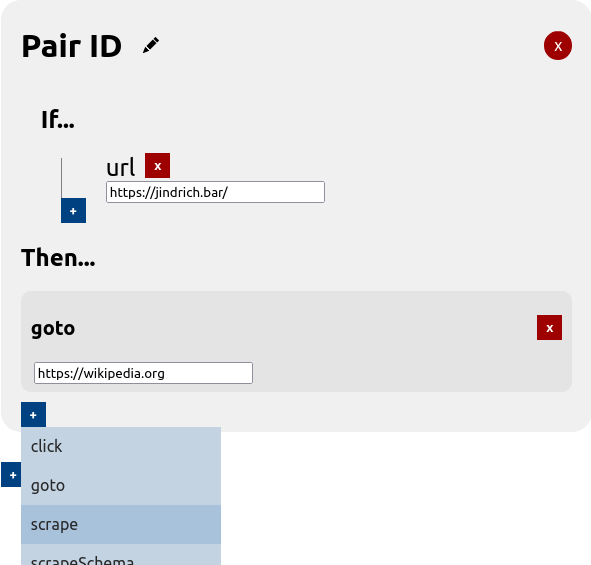
\includegraphics[width=0.60\textwidth]{./img/tutorial/actions.png}}
    \end{center}
    \caption{Selecting the actions for a pair}\label{fig:tutorialActions}
\end{figure}

The \autoref{fig:tutorialActions} shows the process of adding new actions to the action sequence corresponding to the pair.

Selecting an action from the dropdown menu results in inserting a new action expression into the action sequence.
The action expression is defined by the action type and optional parameters for the action - e.g. the \texttt{'click'} action requires a \texttt{'selector'} parameter,
the \texttt{'goto'} action requires a \texttt{'url'} parameter etc.

The \textit{Editor} application suggests the required parameters for the individual actions to enhance the user experience and avoid errors.

While the \texttt{wbr-interpret} module provides support for all the \textit{Playwright's} \textit{Page} methods, the \textit{Editor} application supports only a subset of the most common actions.

\subsubsection{Testing the automation}

After creating a new automation, the user can test run the automation by clicking the \texttt{'Run'} button in the top left part of the screen.

This executes the automation, displaying the execution progress in the remote browser window on the right side of the screen.
Additional information about the execution is displayed in the console below the browser window.
To further facilitate the automation debugging, the \textit{Editor} also highlights the currently matched pair in the workflow definition section.

To ensure consistency, any update to the workflow definition made during the workflow execution will stop the automation execution.

\begin{figure}[!h]
    \begin{center}
        \fbox{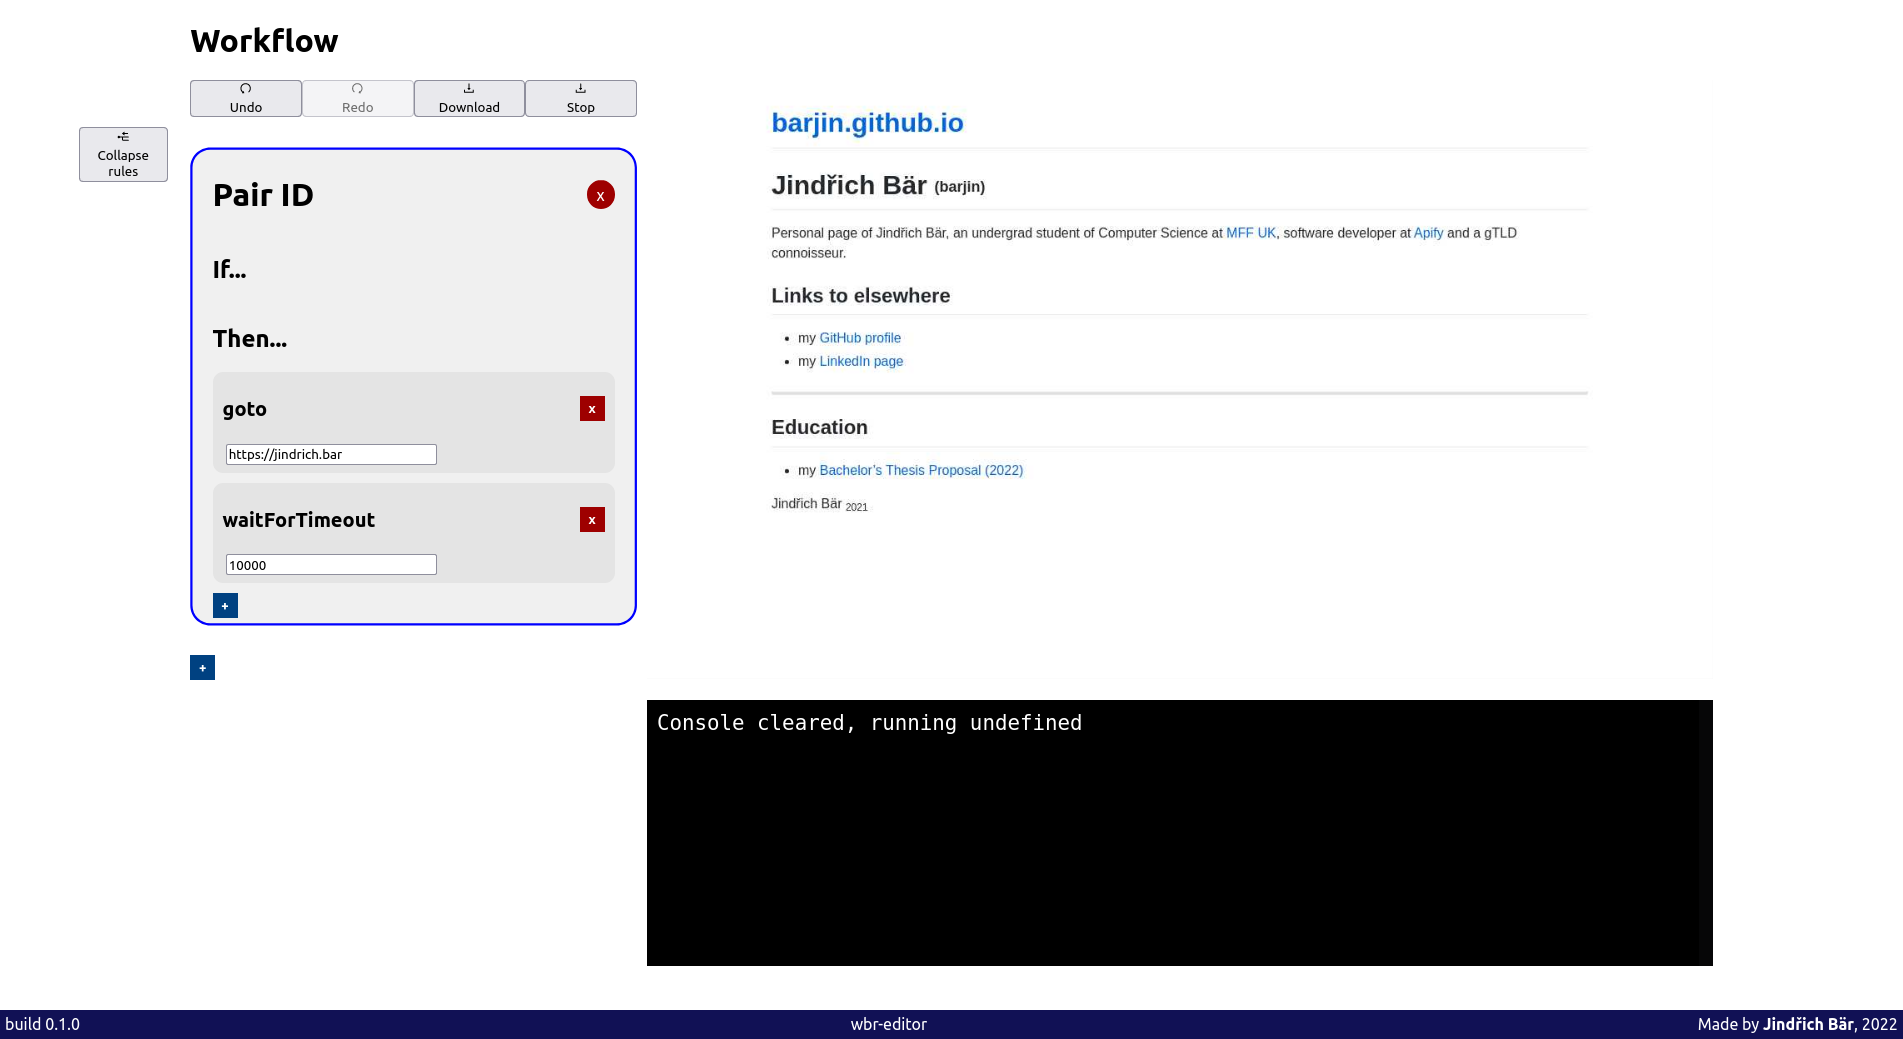
\includegraphics[width=0.8\textwidth]{./img/tutorial/execution.png}}
    \end{center}
    \caption{Execution of a simple workflow}
\end{figure}